\chapter{Previous Work}
\label{ch:prev}
\vspace{-0.8cm}
\section{Sequential Equivalence Checking}
As an important component of formal verification for sequential circuits, SEC techniques 
have been developed over decades and widely utilized in both academia and industry. 
The specification of a sequential circuit can be modeled as a (golden model) state machine;
SEC is performed to compare the functionality between the circuit for test and the golden one.
% The n\"aive method to implement SEC is: preload both circuits to the same initial states, 
% and assign their primary inputs to the same values during all clock-cycles.
% This method needs to be operated along with state space traversal,  therefore it is 
% less efficient. Moreover,  most SEC only check the primary outputs/inputs consistency 
% and does not require the 1:1 state correspondence,  so state space traversal is not always necessary.
One way to implement SEC is to create a miter with two circuits to be verified, then 
prove that there exists no sequence of inputs that generates different outputs.

Researchers proposed improvements by using Boolean functions to represent 
a set of states/transitions \cite{coudert2003unified, coudert1990verification},  or by dividing the sequential circuit
into a smaller subcircuit and remodeling the FSM to conditional FSMs \cite{khasidashvili2004theoretical}. IBM created a toolset with 
interfaces that focuses on only the designated initial states and removes redundancies in state space \cite{baumgartner2007scalable}.

Another direction to improve SEC algorithms is to avoid using state space traversal. 
The forward retiming method \cite{van1998sequential} and time-frame merging \cite{stoffel1997record} 
all work on an array of time-frames,  with the assistance of combinational equivalence checking (CEC)
techniques. These techniques require structural similarities between the two circuits.

The most significant difference of sequential circuits from combinational circuits is 
that the outputs of the circuit depend not only 
on the primary inputs, but also on current state. 
The behavioral difference reflects on the structural design of circuits and in 
the existence of memory components such as latches and flip-flops.
In order to test certain properties on some signals across multiple clock-cycles,
the most straightforward method is to propagate those signals throughout 
all clock-cycles. Moreover, for formal verification, all signals on all paths from the circuit
need to be propagated through multiple clock-cycles.
This indicates a time-to-space conversion, where 
 the combinational part of circuit
is copied over several time-frames then connected together.
The procedure is called {\it unrolling} of a sequential circuit, as 
Figure \ref{fig:unrolling} shows.

\begin{figure}[tbp]
\centerline{
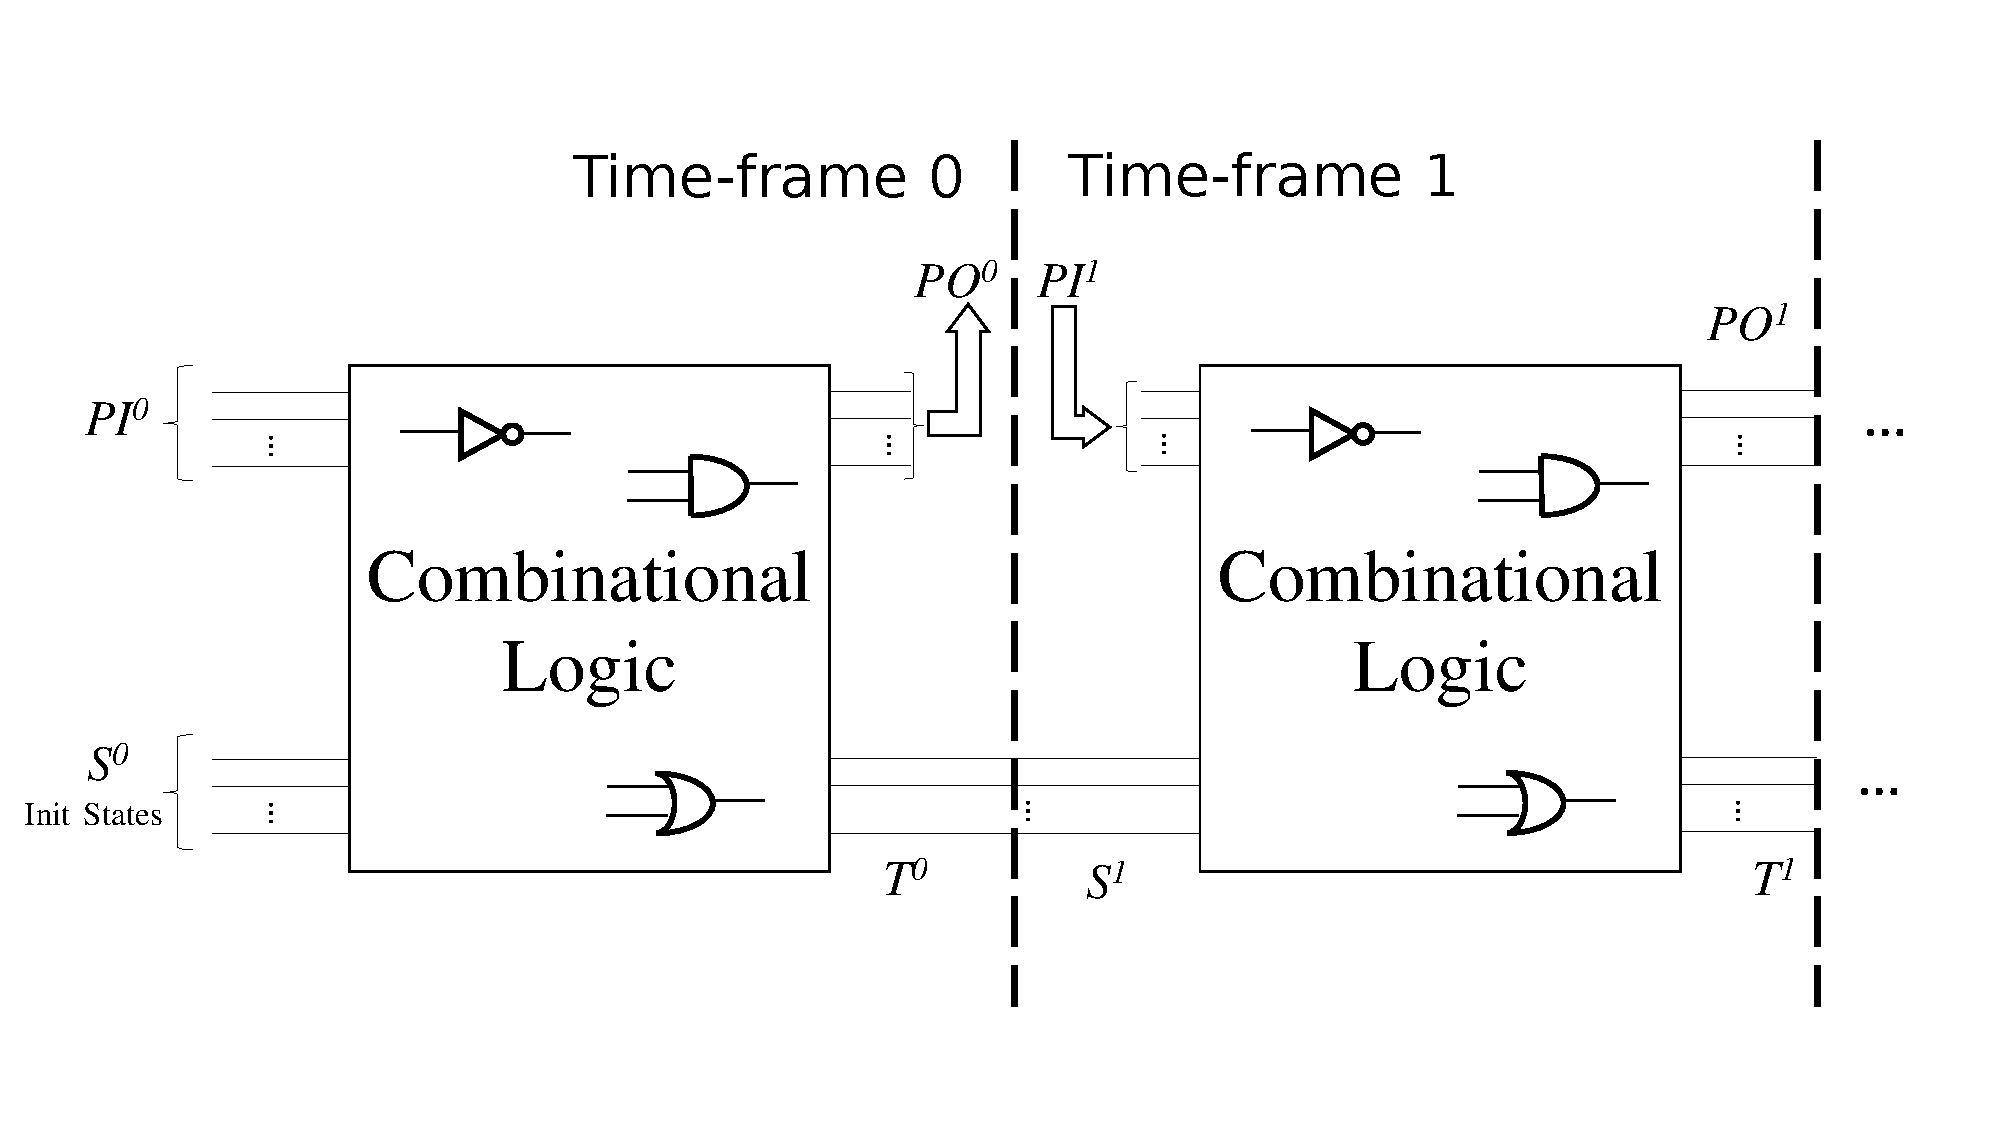
\includegraphics[width=\textwidth]{newfig/unroll.pdf}
}
\caption{The unrolling of a sequential circuit.}
\label{fig:unrolling}
\end{figure}

Unrolling provides a way to transform a sequential circuit into a combinational 
circuit. Therefore,  methods which can be applied to combinational circuit 
verification are also suitable for unrolled sequential circuits. The canonical 
graphical representation of the combinational circuit after unrolling is also 
the canonical representation of the original sequential circuit. For the sequential 
equivalence checking problem, we can also unroll the circuit to be verified and the 
specification to combinational ones, and then perform combinational equivalence checking
techniques \cite{savoj2010combinational}. In the following part we review research and techniques which 
can be applied to unrolled sequential circuits.

\subsection{Canonical Decision Diagrams}
The decision diagrams (DDs) are optimized data structures which can significantly accelerate formal verification.
The most fundamental DD is the Binary DD (BDD), which originates from the 
Shannon's expansion:
\begin{equation}
f(x, y, \dots) = x f_x + x' f_{x'}
\end{equation}
where $f_x = f(x = 1)$ and $f_{x'} = f(x = 0)$ denote the positive and
negative co-factors of $f$ {\it w.r.t.} $x$, respectively.
A BDD is usually represented as a binary tree.
Its ordered and reduced form, the Reduced Ordered Binary Decision Diagram (ROBBD)
\cite{BRYA86}, was the first significant contribution because of its canonicity.  
ROBDDs represent a Boolean function as an
implicit set of points on a canonical directed acyclic graph
(DAG). Manipulation of Boolean functions can then be carried out as
composition operations on their respective DAGs. An example of ROBDD is shown as Figure \ref{fig:BDD}.

Following BDDs,  variants of Shannon's decomposition principle
were explored to develop other functional decision diagrams such as
 FDDs \cite{okfdd}, ADDs \cite{add}, MTBDDs \cite{mtbdd}, and their hybrid 
edge-valued counterparts, HDDs \cite{hdd} and EVBDDs \cite{evbdd}. 
Zero-suppressed BDDs (ZDDs) \cite{minato1993zero,minato1994calculation} use the if-then-else branches
to represent the existence of variables in a cube, and result in lower 
space complexity. They can be used to represent polynomials with integer coefficients.

\begin{figure}[bp]
\centerline{
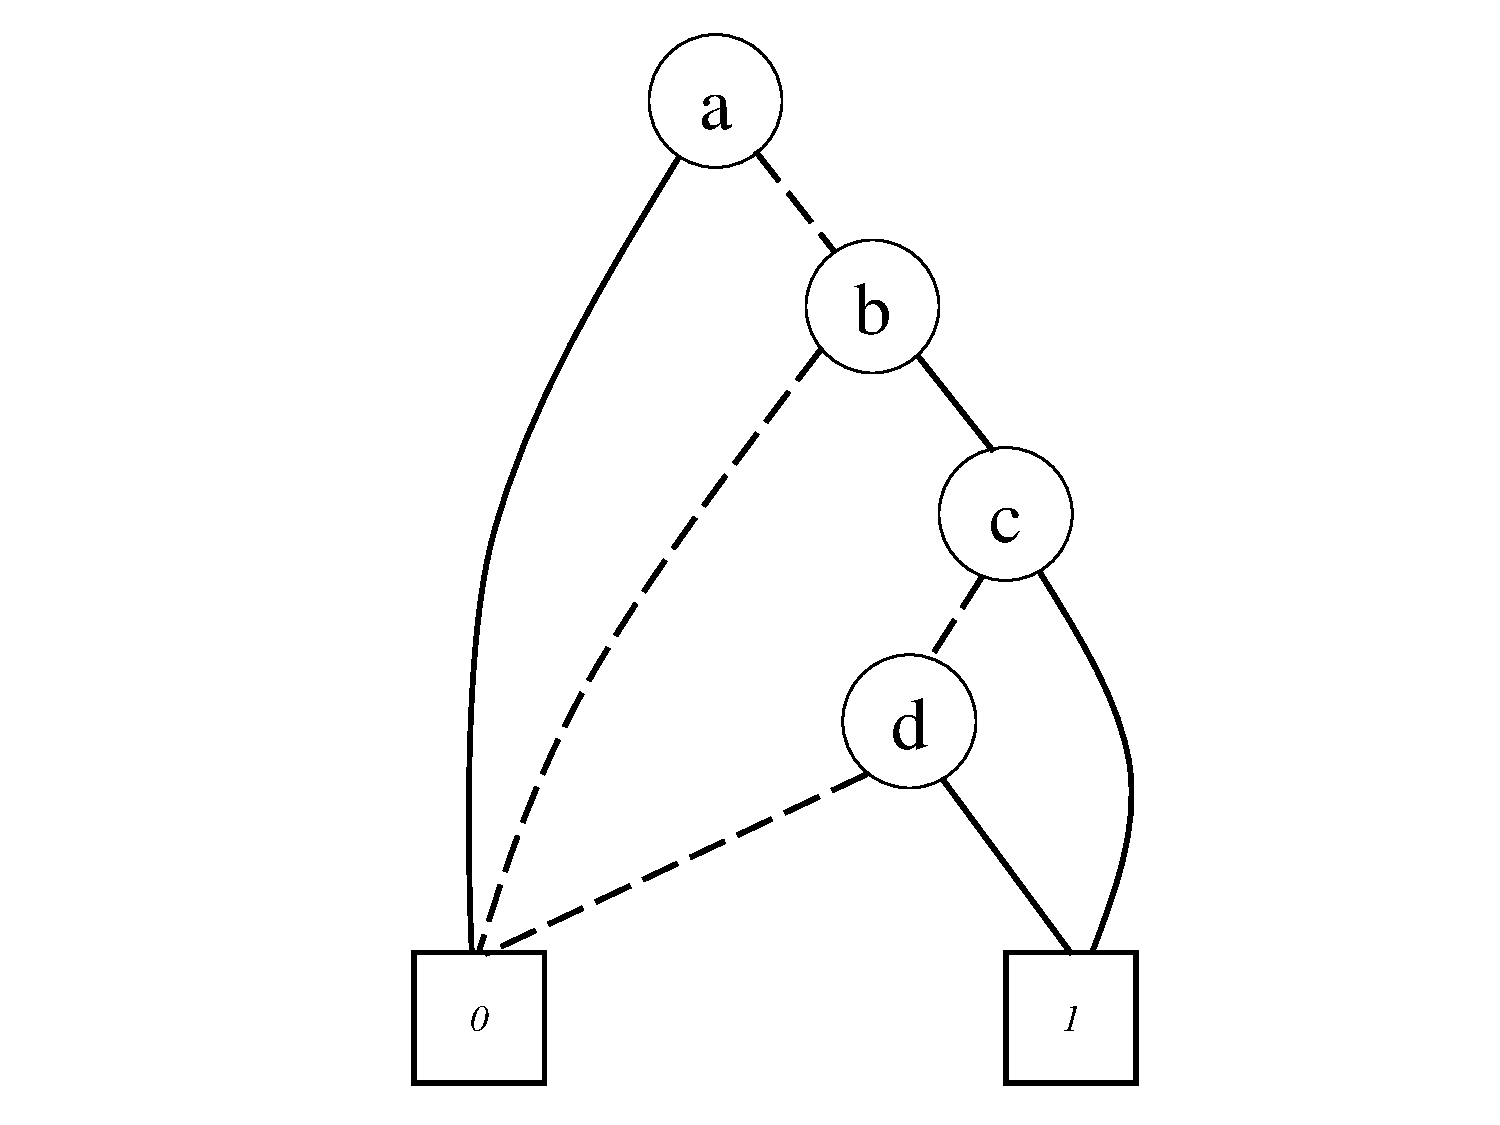
\includegraphics[width=0.45\textwidth]{newfig/BDD.pdf}
}
\caption{ROBDD representing Boolean function $\neg a \land b \land (c\lor d)$ with order $a>b>c>d$.}
\label{fig:BDD}
\end{figure}

The DDs above are all based on bit-level operations. Even in the {\it Word-Level Decision Diagrams}
\cite{WLS}, the decomposition is still point-wise, binary, 
w.r.t. each Boolean variable. These representations do not
serve the purpose of word-level abstraction from bit-level
representations. 

Binary Moment Diagrams (BMDs) \cite{bmd}, and their derivatives K*BMDs
\cite{kbmd} and *PHDDs \cite{phdd}, perform the decomposition of a {\it linear} function
based on its two moments instead of relying on Boolean decomposition. 
MODDs \cite{modd,modd_tcomp} are a DAG representation of the
characteristic function of a circuit over Galois fields $\Fkk$. 
However, MODDs fails to compactly represent large circuits.


Taylor Expansion Diagrams (TEDs) \cite{ted_tcomp} are a
word-level canonical representation of a {\it polynomial expression},
based on the Taylor's series expansion of a polynomial. However, they do
not represent a {\it polynomial function} canonically. 

The use of DDs in traditional formal verification has a lot of advantages. 
For example, DD-based model checking is very efficient as long as the DDs of sequential 
circuit can be setup. The existence of violating states in constructed DDs 
immediately deduces the violation of property. However, when the design gets
larger and larger, the time and space cost of building and storing the diagram 
increases rapidly. In our experiment of verifying a $k$-bit arithmetic circuit 
using ZDDs, when $k$ is larger than 100, the construction of ZDDs occupies 
over $99\%$ runtime of the whole procedure.
\subsection{Combinational Equivalence Checking Techniques}
The CEC problem can be solved using various methods.
Besides using canonical DDs (BDDs
\cite{BRYA86} and their word-level variants \cite{WLS}),
noncanonical representations such as And-Invert-Graph-based (AIG-based) reductions 
\cite{AIG:2002,alanmi:cec:iccad2006} are also very effective. 
Solvers for satisfiability problems (SAT) are good candidates to solve CEC problems,
as long as the miter of two circuits can be described using conjunctive normal form (CNF)
formulas. Applications of SAT on CEC include circuit-SAT solvers \cite{csat}, etc.
If the circuits being compared are structurally highly similar, AIG and circuit-SAT-based
approaches are known to be efficient.
However, when the circuits are functionally equivalent but structurally very dissimilar, none of the 
  contemporary techniques, including quantifier-free bit-vector 
  (QF-BV) theory-based SMT-solvers \cite{Cryptol:fmcad09},
  offer a practical solution.    


Recently integer polynomial based techniques \cite{ciesielski2014function,rolf:date16} have been proposed  to verify the functional 
correctness of integer arithmetic circuits. Their approach formulates the output signature as a polynomial function 
with binary variables and integer coefficients, then rewrites the polynomial by substituting gate output with gate 
inputs. After going through the backward rewriting procedure,  the polynomial
will be composed by only input variables. Then the polynomial is converted to a canonical representation, and compared
with a designated input signature. If they are equivalent, then the arithmetic circuit is successfully verified.
This approach incurs polynomial term explosion during the backward rewriting. The authors proposed a heuristic
to levelize the arithmetic circuit, and substitute several gates' variables at the same time to minimize the risk. However, 
the heuristic proved to be less effective when the inner symmetry of the circuit structure is missing.

% To conclude, automatic formal verification of large {\it
%     custom-designed modulo-arithmetic circuits} largely remains
%   unsolved today.
  
\section{Symbolic Model Checking and Abstraction Refinement}
Model checking is a way to verify certain safety and liveness properties 
in sequential circuits. Symbolic model checking, which avoids using explicit state encoding,
provides more flexibility to reduce the state space and enhance the 
efficiency of model checkers. The implementations of symbolic model checking 
require canonical DDs or SAT solvers \cite{burch1990sequential,burch1991representing,biere1999symbolic}.

Abstraction is a technique to reduce the state space representation by combining states with similar 
characteristics. Sometimes it can effectively lower the number of states that require analysis by orders of magnitude,
without affecting the properties we need to verify. Model checkers then utilize abstracted models 
with interpolation \cite{mcmillan2003interpolation,mcmillan:cav06}.
At first, abstraction was done manually by designers. Clarke {\it et al.} \cite{clarke2000counterexample}
proposed a BDD-based automated abstraction by removing spurious paths from analysis of counterexamples. 
Zhang {\it et al.} \cite{zhang2005design} proposed another abstraction method based on CNF-SAT.
It implemented latch abstraction by removing "irrelevant" latches by analyzing the 
UNSAT core from the $k$-BMC. Jain {\it et al.} \cite{jain2005word} improved the abstraction refinement technique of \cite{clarke2000counterexample},
where they use CNF-SAT to perform the refinement instead of using BDDs. The new approach is applied to verify RTL Verilog
and was known to be successful.

The $k$-BMC with interpolation is a purely incremental model-checking approach, and the interpolation procedure relies
on UNSAT core analysis. To overcome these weaknesses, a hybrid model checker called IC3 is developed 
\cite{bradley2011sat,bradley2011incremental}. IC3 works incrementally to find inductive subclauses
of negations of reached states, meanwhile it is monolithic when computing overapproximations to sets of reachable
states within $1,2,\dots,k$ steps. It is proved to be more efficient than interpolation-based model checking,
although using similar mechanisms.

The above techniques have limitations: they all rely on bit-level information from 
the circuit, which prevents them from being applied to circuits with large datapaths.
Meanwhile, their implementation relies on SAT/BDDs, which is an extension of Boolean 
functions and not compatible with other forms of constraints.

\section{Word-level Techniques Applied to Sequential Circuit Synthesis and Validation}
To better verify word-level designs, word-level verification techniques have been 
explored in recent years. Directly translating bit-vector problems to bit-level 
problems is called {\it bit-blasting}, and usually brings high redundancy and computational complexity in verification.
Attempts to develop pure word-level techniques can be found in
the rich domain of 
theorem proving \cite{arditi:bmd} and bit-vector SMT-solvers
\cite{boolector,cvc3,z3,bitvector98}, automated
decision procedures for Presburger arithmetic \cite{presburger,bultan:mixed_verification}, 
algebraic manipulation techniques 
\cite{devadas:algebraic_manipulation_iccd91}, or the ones based on
term rewriting \cite{AST}, etc.

Polynomial, integer, and other nonlinear representations have also
been researched: Difference Decision Diagrams (DDDs) \cite{ddd-csl99,ddd-mt-98}, interval
diagrams \cite{interval_dd}, interval analysis using polynomials
\cite{polynomial_sanchez99}, {\it etc.} Most of these have found 
application in constraint satisfaction for simulation-based
validation:  \cite{Ritter99,hsat,lpsat,brinkmann:asp-dac,Huang:tcad01,bitvector98}. Among
these, \cite{brinkmann:asp-dac,Huang:tcad01,bitvector98}
have been used to {\it solve} integer modular arithmetic on linear
expressions -- a different application from {\it representing}
finite field modulo-arithmetic on polynomials in a canonical form.   

Uninterpreted function abstraction is also an important category of 
word-level techniques which facilitates word-level model checking.
Usually uninterpreted symbols have no notion of bit-vector-precision. However, these techniques
constrain them 
using functional consistency among the evaluations of word variables
\cite{UF1,UF2,UF3}.


\section{Verification Using Algebraic Geometry}

Symbolic computer algebra techniques have been employed for formal
verification of circuits over $\Z_{2^k}$ and also over
Galois fields $\Fkk$. 
Verification techniques using Gr\"obner bases
\cite{Avrunin:CAV,gbverify:2007,manna:program} are proposed,
but they do not address the problem of high computational complexity to
compute Gr\"obner bases.

Verification of a combinational Galois field arithmetic circuit $C$ against a
polynomial specification $\Func$ has been previously addressed 
\cite{ibm:blueveri,lv:tcad2013,pruss:dac14}. Verification problems in
\cite{ibm:blueveri,lv:tcad2013} are formulated using
Nullstellensatz and decided using the \Grobner basis algorithm.

The paper 
\cite{pruss:dac14} performs verification by deriving a canonical
word-level polynomial representation $\Func$ from the circuit $C$. Their
approach views any arbitrary Boolean function (circuit) $f: \B^k
\rightarrow \B^k$ as a polynomial function $f: \Fkk \rightarrow \Fkk$,
and derives a canonical polynomial representation $\Func$ over
$\Fkk$. They show that this can be achieved by computing a reduced 
\Grobner basis {\it w.r.t.} an {\it abstraction term order} derived from the
circuit. Subsequently, they propose a \underline{r}efinement of this
\underline{a}bstraction \underline{t}erm \underline{o}rder (called
RATO) that enables them to compute the \Grobner basis of a smaller subset
of polynomials. The authors show that their approach can prove the
correctness of up to 571-bit combinational GF multipliers. 

IBM proposed a method to apply algebraic geometry techniques 
to verifying error coding circuits \cite{BLUEVERI}.
Recent papers \cite{rolf:date16,rolf:FMCAD16} provide a way to utilize 
algebraic geometry and GB-based symbolic computing and perform 
equivalence checking on integer arithmetic circuits and floating-point 
arithmetic circuits, respectively.

The use of algebraic geometry
for sequential circuit verification and symbolic model checking has
been presented before. Avrunin presented the
concept of symbolic MC using algebraic geometry in
\cite{Avrunin:CAV}. Later, in \cite{vardi-iasted07}, Vardi presented
GB-algorithms for CTL, LTL, and 
bounded MC over Boolean rings. However, these approaches are a
straightforward transformation of the problem to {\it bit-level}
Boolean GB engines which are used in lieu of BDDs or SAT solvers. All
the concepts of word-level reachability, abstraction-refinement using
interpolation or UNSAT cores, etc., that we desire were not the focus of
\cite{Avrunin:CAV,vardi-iasted07}. 

\section{Concluding Remarks}
From the investigation of previous work, techniques are to be researched that 
can perform the FSM traversal at word level to verify a property excluding spurious 
faults. Meanwhile, many abstraction refinement techniques utilize information from UNSAT cores.
We propose to solve these problems in the context of word-level verification,
with data representation, abstraction, and algorithm execution all carried out 
at word level.

In this dissertation, we propose a purely word-level reachability analysis approach, which has never been done before.
We achieve this by modeling the transition relations, states and the traversal algorithm at word level.
We borrow inspirations from \cite{tim:phd,gao:qe-gf-gb} to perform state space abstraction.
Moreover, we demonstrate applications of our proposed approach to sequential arithmetic verification, which has 
not been done before, either.
Finally, we show algebraic geometry analogs of UNSAT cores of polynomial ideals, and describe algorithms
to extract and refine these cores.
